\chapter{Introduction}

The steady advancement of technology
has automated an increasing variety of menial or dangerous tasks
previously performed by humans.
Computer algorithms now trade our stocks,
route our telephone calls and packages,
and fly our planes,
while simple machines clean our clothes and wash our dishes.

More complex tasks require complex robots with many
degrees of freedom.
Manipulation tasks, in particular,
present challenges in many areas including
perception, symbolic reasoning, and motion planning.
Successful applications have so far been largely
confined to manufacturing domains
whose prescribed and structured environments
allow these challenges to be overcome.

In contrast,
consider the manipulation tasks in Figure~\ref{fig:intro-examples}.
In the first application,
the \textsc{Herb} home robot must retrieve a frozen meal from 
a cluttered countertop
and transfer it into a microwave oven.
In the second,
the \textsc{Chimp} distaster response robot
must clear large pieces of debris from a blocked doorway
in the recent DARPA Robotics Challenge competition.
These multi-step manipulation tasks
require finding motion plans in
high-dimensional, dynamic, semi-structured spaces
under significant resource constraints (e.g. time or energy).
State-of-the-art approaches can not yet handle these
planning problems quickly and reliably.

%\begin{figure}
\begin{marginfigure}
%{\setlength{\offsetpage}{0.5in}
%\begin{widepage}
   \centering
   \subfloat[
      The \textsc{Herb} assistance robot
         moves a frozen meal into a microwave oven.
   ]{%
      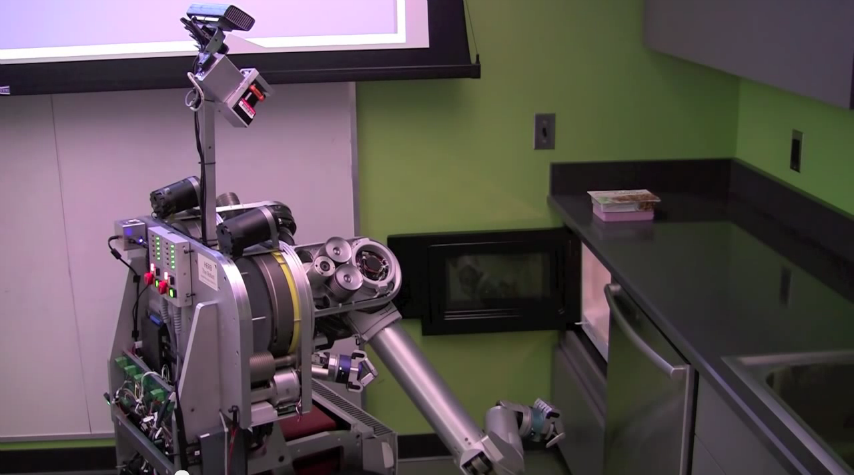
\includegraphics[width=\textwidth]{figs/herb-microwave-intro.png}
   }
   \vspace{-0.1in}
   \subfloat[
      The \textsc{Chimp} distaster response robot
      clears debris from a blocked doorway.
   ]{%
      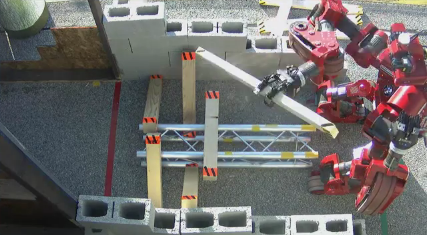
\includegraphics[width=\textwidth]{figs/chimp-debris-overhead.png}
   }
   \vspace{0.02in}
   \caption{This thesis addresses multi-step motion planning
      for manipulation tasks.}
   \label{fig:intro-examples}
%\end{widepage}
%}%offsetpage
%\end{figure}
\end{marginfigure}

%\begin{quote}
\begin{adjustwidth}{0.3in}{0.3in}
\emph{%
This thesis proposes an
efficient motion planning approach
well-suited
to articulated robots
performing recurring multi-step manipulation tasks
in dynamic, semi-structured environments.
}
\end{adjustwidth}
%\end{quote}

To address this problem in depth,
this thesis focuses on
efficient kinematic planning approaches
to coupled manipulation tasks consisting of several (2-5) steps
as formuated in Chapter~\ref{chap:proposal-framework}.
We don't consider uncertainty
or feedback to symbolic planners,
and we focus primarily on sequential planning and execution.
We consider our approach complementary to
hybrid and interleaved planners,
as well as approaches which learn heuristics.

\section*{Challenges to Efficient Manipulation Planning}

There are three principal challenges inherent in
human-scale manipulation tasks,
such as those from Table~\ref{tab:challenges-insights},
which render the planning problem difficult.
We survey them here.

\begin{table*}[t]
   \centering
   \begin{tabular}{cc}
      \toprule
      Challenges & Insights \\
      \midrule
      Capturing Planning/Execution Tradeoff
         & Minimize Ensemble Effort on Explicit Graphs \\
      Incongruent Sub-Problems Impede Reuse
         & Identify and Exploit Multi-Set Structure \\
      Coupled Steps Require Long-Horizon Plans
         & Comprehensive Sub-Problem Planning \\
      \bottomrule
   \end{tabular}
   \caption[][0.2in]{Challenges and Insights}
   \label{tab:challenges-insights}
\end{table*}

\subsection*{Challenge 1:
   Capturing the Planning vs. Execution Tradeoff}

\begin{figure*}[t]
   \centering
   \subfloat[Planetary exploration, cost = execution effort]{%
      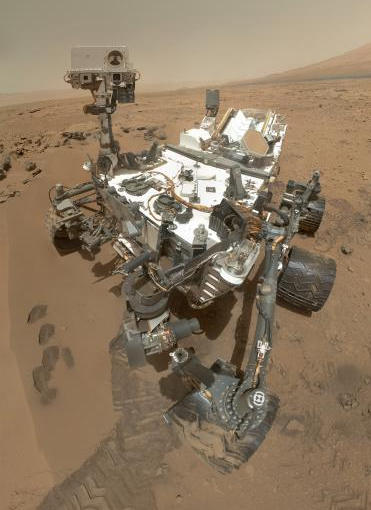
\includegraphics[height=2in]{figs/curiosity-rover.png}%
   }
   \subfloat[Manipulation tasks on the \textsc{Herb} and 
         and \textsc{Chimp} robots,
         cost = planning effort + execution effort]{%
      \includegraphics{build/intro-cost-herb}
      \includegraphics{build/intro-cost-chimp}
   }
   \subfloat[Automated theorem proving,
         cost = planning effort]{
      \fbox{\scriptsize
         \begin{minipage}[b]{1.5in - 2\fboxsep}
            Axioms:\\
            - Axiom 1: $f(1,x) = x$ \\
            - Axiom 2: $u(x,y) = u(y,x)$ \\
            - Axiom 3: $u(1,a) = a$ \\
            \vspace{0.1in}
            Goal Theorem: \\
            - $u(a, f(a,b) = f(a,b)$ \\
            \vspace{0.1in}
            Proof: \\
            \vspace{0.1in}
            Lemma 1: \\
            - $u(z, f(a,z)) = f(a,z)$ \\
            $= u(f(a,z),z)$ by Axiom 2 \\
            $= u(f(a,z), f(1,z))$ by Axiom 1 \\
            \vspace{0.1in}
            Theorem 1: \\
            $\dots$
         \end{minipage}
      }
   }
   \caption[][0.2in]{In many planning domains,
      either planning effort or execution effort is most important
      to minimize.
      For manipulation tasks,
      the \textsc{Herb}
      and \textsc{Chimp}
      incur comparable cost (e.g. time or energy)
      during planning and execution.
      It is therefore important for planning approaches
      to accurately model and reason about this tradeoff.
      }
   \label{fig:plan-exec-cost}
\end{figure*}

%\footnotetext{Image Credit:
%   NASA / JPL-Caltech / Malin Space Science Systems}

Manipulation robots must be resource-efficient.
If a home robot takes thirty minutes to clear a table,
or a disaster response robot exhausts its battery ten minutes
into its mission,
these robots will not see widespread use.
A robot expends two types of effort.
First, it must allocate computation to \emph{plan}
a sequence of motions that will acheive the task.
Second, it must \emph{execute} these motions using its actuators.
Typically, there is a tradeoff between these two;
spending more effort planning produces solutions that are
cheaper to execute.

Consider the spectrum of planning domains
in Figure~\ref{fig:plan-exec-cost}.
In many types of problems,
such as planetary exploration,
execution resources are most scarce,
and therefore the optimality of the solution is most imporant.
On the other hand,
in domains such as automated theorem proving,
the quality of the solution is less important;
planners are instead designed to find a feasible solution quickly.

In manipulation tasks,
both types of efficiency are equally important;
metrics such as time or energy use are only meaningful
when applied across the entire task (from assignment to completion).
In fact, measured in either time or energy,
robots tend to expend comparable effort on each.
For example, at the DRC Trials,
the CHIMP robot spent an average of 140.6 s planning,
and 373.6 s executing those plans
(with very slow execution speeds for safety).
\cdnote{Get timing examples for a HERB example as well.}
Therefore,
manipulation task planners must be able to reason about
the important tradeoff between these two types of effort.

\subsection*{Challenge 2: Incongruent Sub-Problems Impede Reuse}

\begin{figure*}[t]
   \centering
   \subfloat[Fixed worlds (multi-query)]{%
      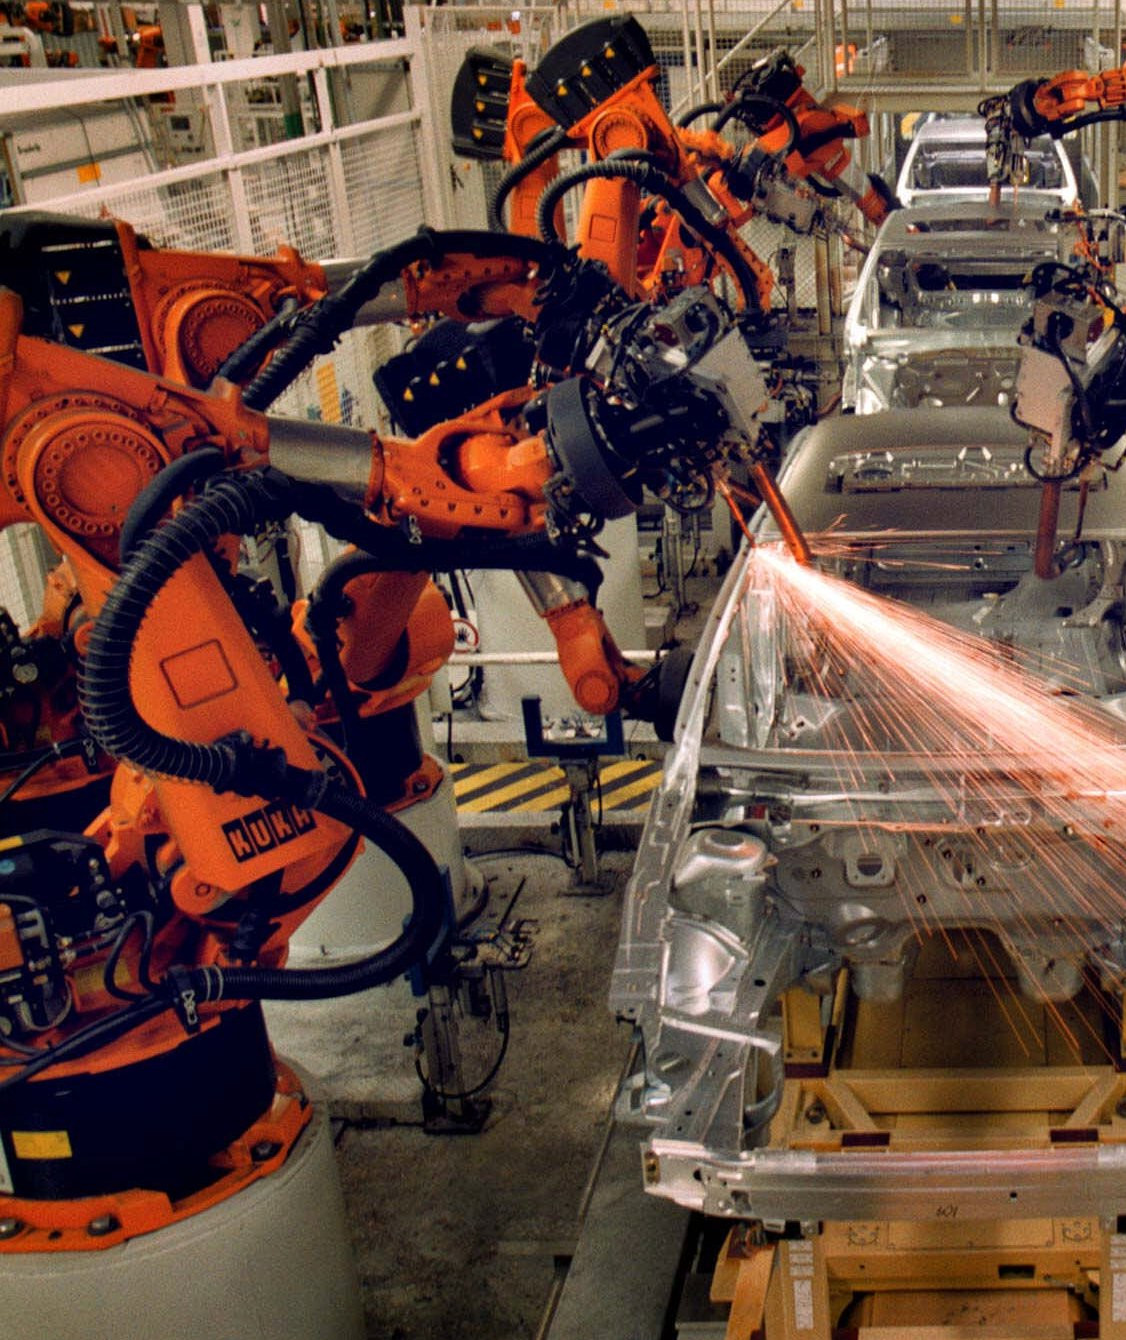
\includegraphics[height=1.6in]{figs/car-robots.jpg}%
   }%
   \;%
   \subfloat[A multi-step problem.]{%
      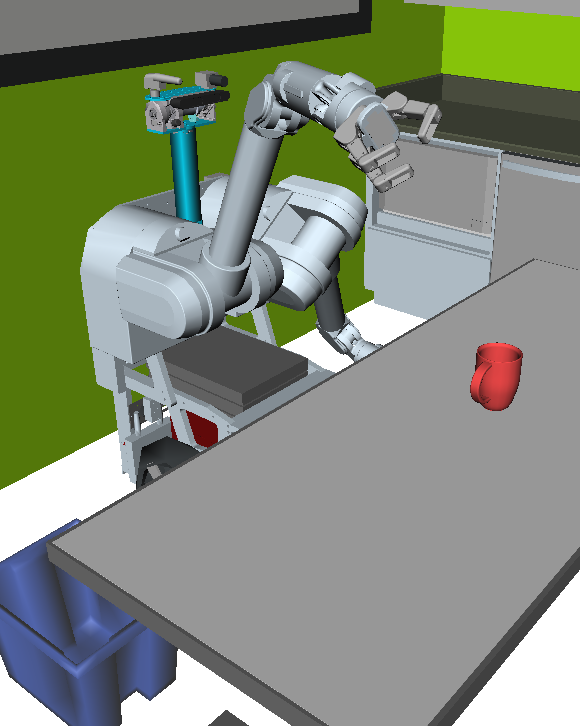
\includegraphics[height=1.6in]{figs/testherb-b.png}%
      \,%
      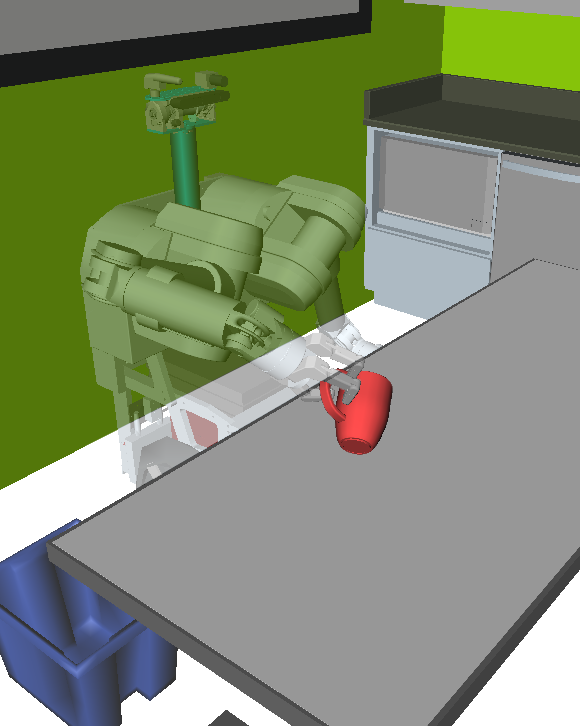
\includegraphics[height=1.6in]{figs/testherb-c.png}%
      \,%
      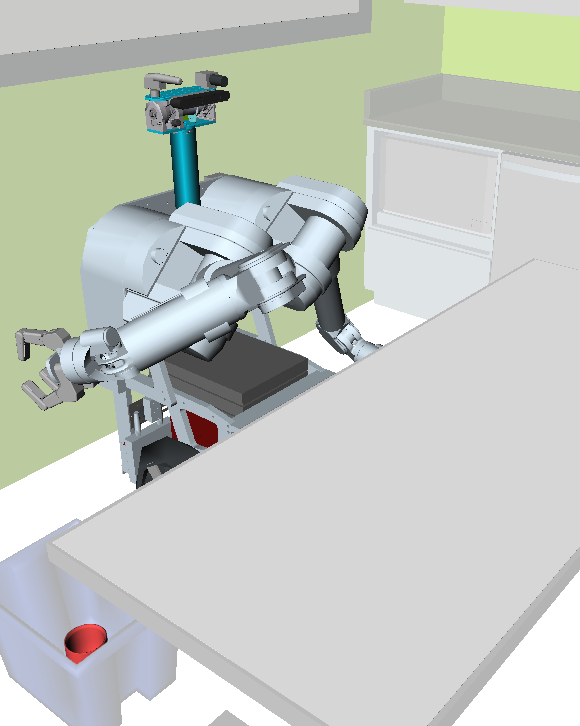
\includegraphics[height=1.6in]{figs/testherb-d.png}%
   }%
   \;%
   \subfloat[Random worlds (single-query)]{%
      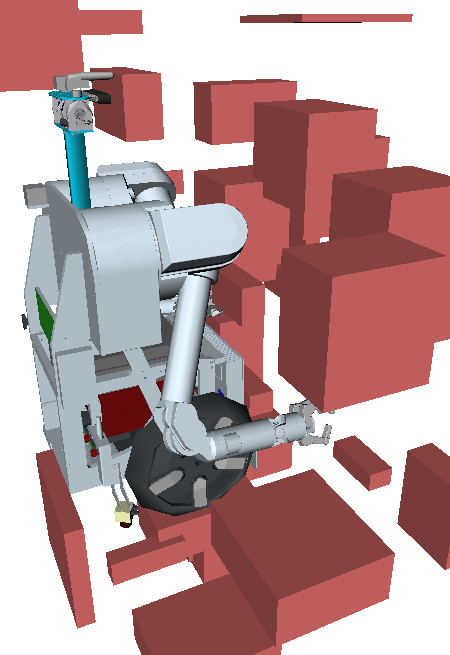
\includegraphics[height=1.6in]{figs/herb-random-world.jpg}%
   }
   \caption[][0.2in]{\textsc{Herb} plans for a simple manipulation task
      to grasp, transfer, and drop a mug from a table into a bin
      before returning to an end configuration.
      Each sub-problem requires a path in a distinct free subset of
      configuration space.}
   \label{fig:intro-multi-part}
\end{figure*}

Because planning effort is such an important factor in
manipulation task efficiency,
it's important to consider approaches which minimize computation
across multiple planning queries.
This is especially important in high-dimensional spaces,
where planning costs are dominated by \emph{validity checking} --
e.g. checking whether configurations are free from collision.
However, the structure of manipulation problems
makes it difficult to apply common approaches.

Consider the motion planning problems in
Figure~\ref{fig:intro-multi-part}.
In the first case,
an industrial robot repeatedly addresses the same scene;
\emph{multi-query} approaches such as the
Probabalistic RoadMap\cite{kavrakietal1996prm}
have proven effective at facilitating reuse in such cases.
However,
autonomous manipulation robots perform tasks
in dynamic, semi-structured environments.
Further,
during each step of a manipulation plan,
the valid subset of configuration space changes
as objects are grasped and moved,
making it difficult to apply roadmap approaches.

At the other extreme,
a robot addressing a set of different random worlds
are best served by \emph{single-query} approaches
which build a unique graph structure ``from scratch''
for each problem they solve.
Applying such approaches to multi-step manipulation tasks
leads to inefficiency in planning
as computation is not reused between queries.

Manipulation sub-problems do have structure.
Since they occupy this middle ground between
fixed and random environments,
it's essential that planning approaches
find a way to reuse computation effectively
between inconguent sub-problems.

\subsection*{Challenge 3: Coupled Steps Require Long-Horizon Plans}

\begin{figure}[t]
   \centering
   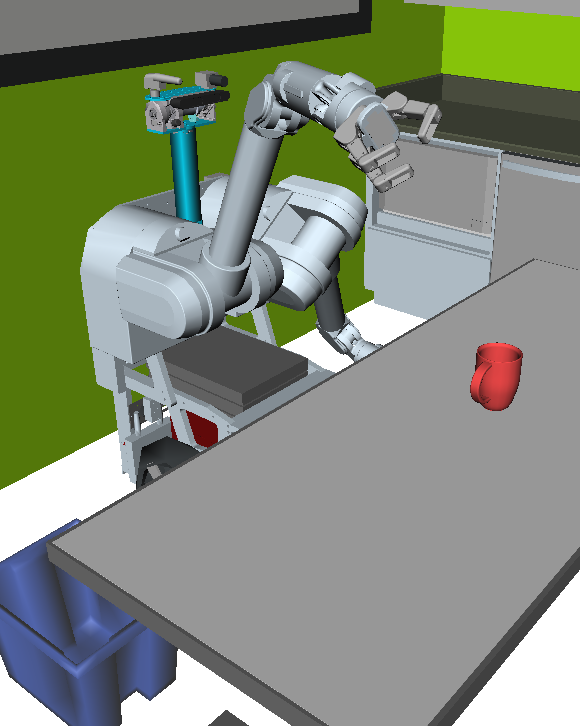
\includegraphics[height=1.4in]{figs/testherb-b.png}%
   \quad%
   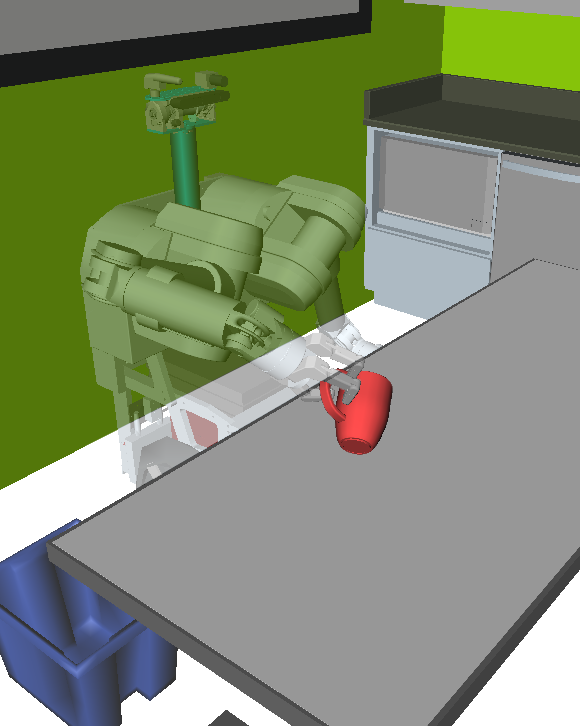
\includegraphics[height=1.4in]{figs/testherb-c.png}%
   \quad%
   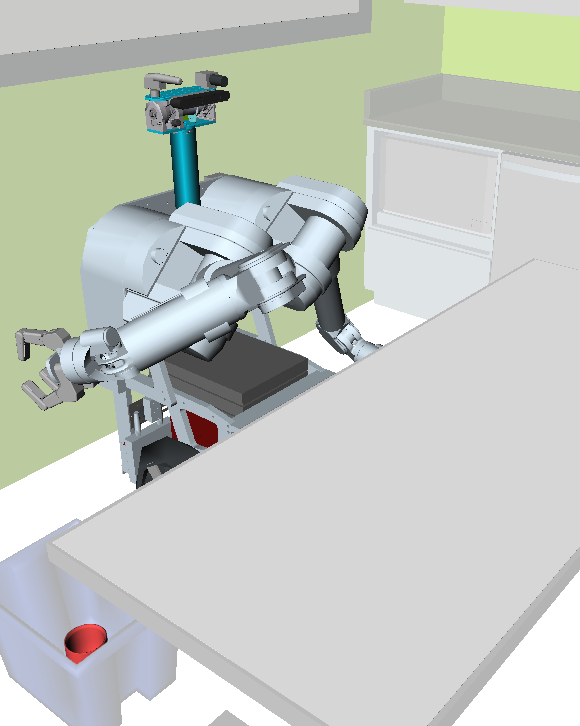
\includegraphics[height=1.4in]{figs/testherb-d.png}
   
   \includegraphics{build/intro-subprob-cspace}
   \caption{Manipulation sub-problems
      within incongruous free subsets
      of configuration space.}
\end{figure}

Not only does the structure of manipulation tasks
impede planner reuse between sub-problems,
but it also necessitates long-horizon plans to ensure robustness.
For example,
consider sequentially planning for the task in
Figure~\ref{fig:intro-multi-part}.
The interfaces between these three steps lie on continuous manifolds.
A choice made by an early planning step
-- e.g. what arm configuration or object grasp to use --
often renders a subsequent part either difficult to plan,
costly to execute, or impossible altogether.
We say that such sub-problems are \emph{coupled}.

We therefore might endeavor to plan for all steps
simultaneously before execution.
Indeed,
many motion planners are designed to take as input
start and goal sets.
We might hope that we can delegate each task sub-problem to
separate such planner instances,
and provide each with specifications for their corresponding
root sets.
However,
a customary planning request takes an \emph{any-to-any} form
(i.e. from \emph{any} start to \emph{any} goal configuration).
Clearly, without coordination,
the juxtaposed solution paths will not be continuous.

\section*{Key Insights to Our Approach}

While these three challenges make efficient
manipulation task planning a difficult problem,
we identify three corresponding and complementary
key insights to address them.
We apply our insights to graph- and roadmap-based planners
as summarized in Table~\ref{table:intro-algorithms}.
A more detailed summary and outline of the structure of
manipulation task planning is presented in
Chapter~\ref{chap:proposal-framework}.
%along with a summary of prior work on the problem.

\begin{table*}[t]
   \centering
   {\renewcommand{\arraystretch}{1.1}
   \begin{tabular}{clcccc}
   \toprule
   {\bf Ch.} & Algorithm & Problem & Representation & Opt-Plan & Multi-Set \\
   \midrule
   & A$^*$ Search \citep{hart1968astar} & Graph & Implicit & No & No \\
   & Weighted A$^*$ Search & Graph & Implicit & Partial & No \\
   & Experience Graphs \citep{phillips2012egraphs} & Graph & Implicit & Partial & Partial \\
   & BUGSY \citep{ruml2007bugsy} & Graph & Implicit & Yes & No \\
    \ref{chap:e8}
      & {\bf E$^8$ Search}
      & {\bf Graph} & {\bf Explicit} & {\bf Yes} & {\bf No} \\
   \midrule
   & Lazy PRM \citep{bohlin2000lazyprm} & $\mathcal{C}$-space & Roadmap (Explicit) & No & No \\
   & Dynamic Planner \citep{jaillet2004dynamicprm} & $\mathcal{C}$-space & Roadmap (Explicit) & No & Partial \\
   \ref{chap:graphs-in-continuous}
      & {\bf E$^8$-PRM}
      & {\bf $\mathcal{C}$-space} & {\bf Roadmap (Explicit)} & {\bf Yes} & {\bf No} \\
   \ref{chap:multi-set-prm}
      & {\bf Multi-Set PRM}
      & {\bf $\mathcal{C}$-space} & {\bf Roadmap (Explicit)} & {\bf Yes} & {\bf Yes} \\
   \midrule
   \ref{chap:task-planning}
      & {\bf \textsc{Proteus}}
      & {\bf Multi-Step Tasks} & {\bf Multi-Graph (Explicit)} & {\bf Yes} & {\bf Yes} \\
   \bottomrule
   \end{tabular}
   } %arraystretch
   \caption[][0.2in]{Comparison of algorithms.
      The ``Opt-Plan'' column denotes planners which explicitly
      optimize an objective which includes a planning effort term.
      The ``Multi-Set'' column denotes planners which reason about
      common structure between related problems.}
   \label{table:intro-algorithms}
\end{table*}

\subsection*{Insight 1: Minimize Ensemble Effort on Explicit Graphs}

Because the tradeoff between planning and execution effort
is so important for manipulation tasks,
it is important to choose problem representations and design algorithms
which accurately model and exploit this structure.
We make two contributions to this end
as described in Chapter~\ref{chap:e8}.

First,
while graph-based approaches have proven effective at solving
many problems in high-dimensional spaces,
we propose that the planning effort model assumed by
traditional search algorithms (e.g. A*)
may not be well-suited to motion planning problems for articulated
robots.
In particular,
we propose that \emph{explicit} graph representations
allow the planner to more accurately capture the significant
edge evaluation costs inherent in such problems.

Second,
our planning approach explicitly optimizes for both planning
and execution effort
-- what we call the task's \emph{ensemble effort}.
We submit that our approach handles this tradeoff more directly
than ``anytime'' planning approaches.
We apply this reasoning to explicit graphs
with the E$^8$ search algorithm
which determines an effort allocation between planning and execution
in order to minimize total task cost.
%We show how we can use incremental graph search approaches
%to make it super fast.

In order to solve planning problems in continous configuration spaces,
we borrow heavily from roadmap techniques for graph construction.
The application of our ensemble effort algorithm to such roadmaps,
the E$^8$-PRM (Chapter~\ref{chap:graphs-in-continuous}),
maintains efficiency through an
incremental densification approach
motivated by approximating the probabalistic spatial correlation of
$\mathcal{C}_{\mbox{\scriptsize free}}$.
We show that this planner outperforms state-of-the-art
single-query motion planners for several manipulation tasks.

%\begin{figure}[t]
%\begin{widepage}
%\begin{center}
%   \begin{subfigure}[b]{2.0in}
%      \begin{center}
%      \includegraphics{build/intro-cost-axis}
%      \end{center}
%      \caption{Planning vs. Execution Cost}
%   \end{subfigure}%
%   \quad%
%   \begin{subfigure}[b]{2.0in}
%      \begin{center}
%      \includegraphics{build/intro-subprob-axis}
%      \end{center}
%      \caption{Single vs. Multi Query Planners}
%   \end{subfigure}
%   \caption{
%      Our approach considers both explicitly
%      during planning.
%      Our approach enables partial reuse between these parts
%      }
%   \label{fig:ensemble-effort-our-approach}
%\end{center}
%\end{widepage}
%\end{figure}

\subsection*{Insight 2: Identifying and Exploiting Multi-Set
   Structure}

In order to address the important issue of planning computation
reuse between the incongruent sub-problems inherent in manipulation
tasks,
we propose the \emph{multi-set} planning formulation
in Chapter~\ref{chap:multi-set}
which bridges the gap between single-query and multi-query approaches.
We explicitly represent the structure of such problems
through labeled subsets of the robot's configuration space,
as well as set relations between them.
We further demonstrate instances of multi-set structure
in many classes of manipulation problems,
and use the formulation to unify several instances of
prior work aimed at efficiently planning for such tasks.

Next, Chapter~\ref{chap:multi-set-prm}
shows how the multi-set formulation can be used as a
planning effort model
when solving planning queries in related subsets of configuration space.
This planning model can then be inserted directly into the 
E$^8$-PRM to handle multi-step problems.
The resulting algorithm,
the Multi-Set PRM,
uses propositional logic to represent the multi-set structure
algorithmically.

\subsection*{Insight 3: Comprehensive Sub-Problem Planning}

Our last insight addresses how to efficiently decompose a coupled
multi-step manipulation task into individual sub-problems.
For tightly coupled problems,
it is especially important to plan for multiple possibilities.
First, we introduce the \emph{Comprehensive Multi-Root} (CMR) planner
objective (Chapter~\ref{chap:cmr}).
In constrast to the traditional any-to-any objective,
CMR encourages a planner to discover paths between multiple pairs of
roots.
We also show that this objective can be applied greedily
to traditional PRM planners
yielding a provably superior algorithm. 

Second,
we introduce the \textsc{Proteus} task planner
(Chapter~\ref{chap:task-planning})
which combines the three insights into a single planning approach.
The task planner
automatically discovers the multi-set structure in each task
and instantiates a Multi-Set PRM to handle planning queries
for each sub-problem.
It then performs root sampling within each interface manifold
and uses the CMR objective for each query to
efficiently search for a full task plan.

\section*{Evaluation}

Because this thesis presents an integrated set of algorithms
for multi-step manipulation task planning,
we endeavor to place significant emphasis on empirical evaluation
in order to verify the performance of the proposed approach.
See research question \ref{ques:proteus-compare} for more details
about the metrics, baseline approaches, and test platforms
that will be used in these comparisons.
\marginnote{\cdnote{I welcome suggestions from my committee for
appropriate baseline approaches.}}

I refer the reader to Chapter~\ref{chap:proposed} for a summary
of the particular research questions that I propose to answer.
Chief among these questions are the effects of the insights above
on task performance as borne out by these experiments:
\begin{itemize}
\itemsep-3pt
\item The effect of the E$^8$ algorithm's planning vs. execution
   effort tradeoff parameter ($\lambda$)
   compared to weighted/anytime approaches.
\item The effect of the E$^8$-PRM's batching strategy on its efficacy
   as a single-query planner in high-dimensional planning
   problems.
\item The performance of the Multi-Set PRM on problems with various
   amounts of shared structure
   (from fully fixed to fully random environments).
\item The performance of the {\sc Proteus} task planner
   compared to other baseline planners that address multi-step tasks.
\end{itemize}

\section*{Summary of Contributions}

In summary,
I propose the following contributions:
\begin{itemize}
\itemsep-3pt
\item A set of insights into the structure of the
   multi-step manipulation planning problem,
   including the multi-set and comprehensive multi-root (CMR)
   formulations.
\item The E$^8$ graph search algorithm which explicitly minimizes
   both planning and execution effort over explicit graphs.
\item The E$^8$-PRM, an application of E$^8$ to
   $\mathcal{C}$-space roadmaps.
\item The Multi-Set PRM, an instantiation of the E$^8$-PRM
   using the multi-set formulation as a planning effort model.
\item The {\sc Proteus} task planner,
   a sequencing planner which submits queries across steps
   to an instance of the Multi-Set PRM using the CMR objective.
\item The {\tt ompl\_multi\_set\_prm} package
   for the OMPL\citep{sucan2012ompl} sampling-based planning framework
   containing implementations of the E$^8$-PRM and Multi-Set PRM
   algorithms.
\item The {\tt or\_proteus} package for the
   OpenRAVE\citep{diankov2010openrave} simulation framework
   which implements the {\sc Proteus} task planner.
\item An experimental evaluation of the above algorithms against
   state-of-the-art baseline approaches.
\end{itemize}

%{
%\setlength{\offsetpage}{0.75in}
%\begin{figure}[t]
%\begin{widepage}
%\begin{center}
%\begin{tikzpicture}
%
%% axes
%\draw[->,thick] (0,0) -- (0,8); 
%\draw[->,thick] (0,0) -- (12,0);
%\node[rotate=90,align=center] at (-1.0,4)
%   {Challenge 1:\\Task Efficiency};
%\node[align=center] at (6,-1.6)
%   {Challenge 2:\\Sub-Problem Structure};
%
%% y tics
%\draw (-0.2,1) -- (0.2,1);
%\node[rotate=90,align=center] at (-0.64,1)
%   {considers\\[-0.04in]execution cost};
%\draw (-0.2,7) -- (0.2,7);
%\node[rotate=90,align=center] at (-0.8,7)
%   {considers\\[-0.04in]planning and\\[-0.04in]execution cost};
%
%% x tics
%\draw (2,-0.2) -- (2,0.2);
%\node[align=center] at (2,-0.5) {no reuse};
%\draw (6,-0.2) -- (6,0.2);
%\node[align=center] at (6,-0.5) {two-set reuse};
%\draw (10,-0.2) -- (10,0.2);
%\node[align=center] at (10,-0.5) {full reuse};
%
%% algorithms
%\node[draw,ellipse,align=center] at (2,1)
%   {Lazy PRM \cite{bohlin2000lazyprm}};
%
%\node[draw,ellipse,align=center] at (6,1)
%   {\cite{leven2000changing}, \cite{kallman2004dynamicroadmaps},
%   \cite{jaillet2004dynamicprm}};
%
%\node[draw,ellipse,align=center] at (2,7)
%   {E$^8$-PRM\\(Chapter~\ref{chap:e8})};
%
%\node[draw,ellipse,align=center] at (10,7)
%   {Multi-Set PRM\\(Chapter~\ref{chap:multi-set-prm})};
%
%\end{tikzpicture}
%\caption{Graphical outline of $\mathcal{C}$-space planners.
%   \cdnote{Work in progress. I don't really like this as it is.}}
%\label{fig:graphical-outline}
%\end{center}
%\end{widepage}
%\end{figure}
%}

%\begin{figure}
%\begin{widepage}
%   \centering
%   \begin{subfigure}[b]{0.24\textwidth}
%      \begin{center}
%      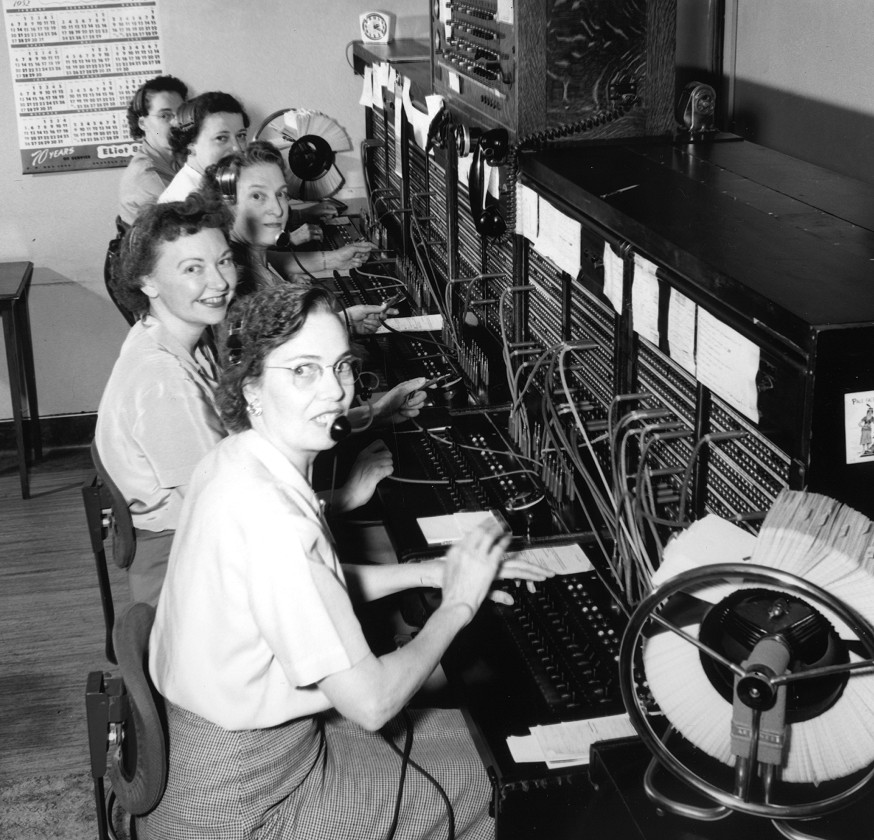
\includegraphics[width=\textwidth]{figs/switchboard.jpg}
%      
%      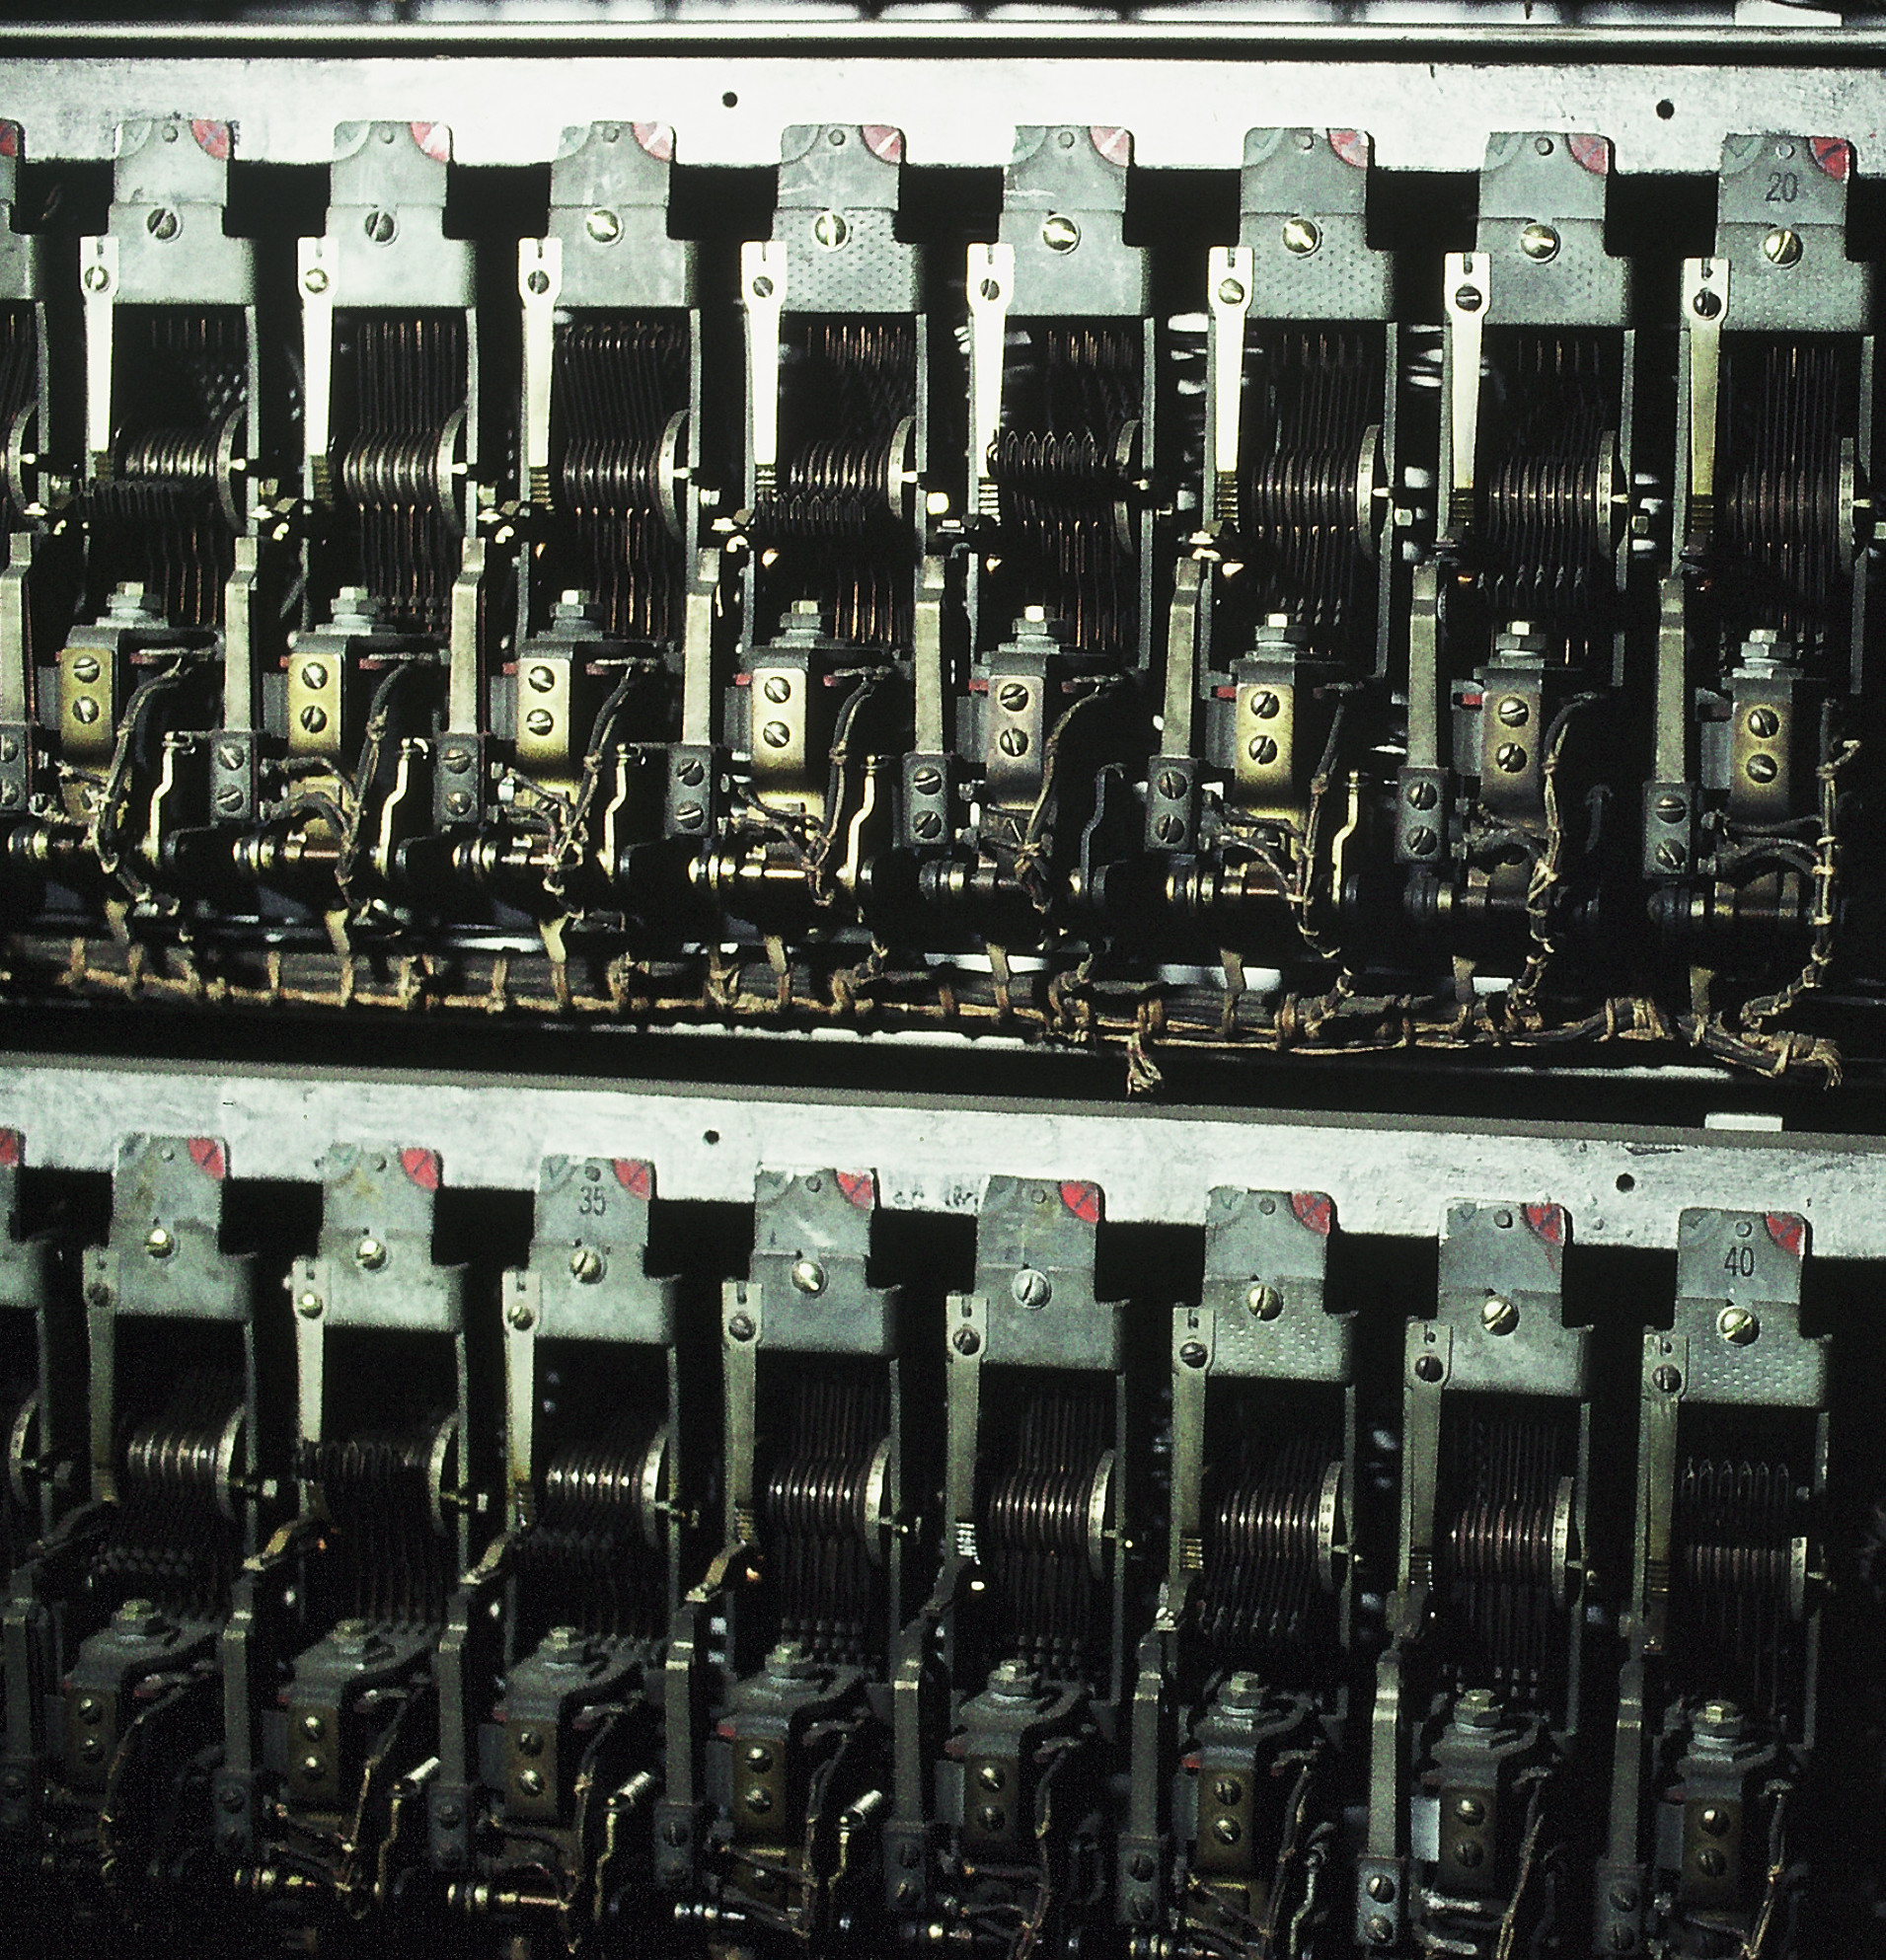
\includegraphics[width=\textwidth]{figs/mech-switches.jpg}
%      \end{center}
%      \caption{Something}
%   \end{subfigure}
%   \begin{subfigure}[b]{0.24\textwidth}
%      \begin{center}
%      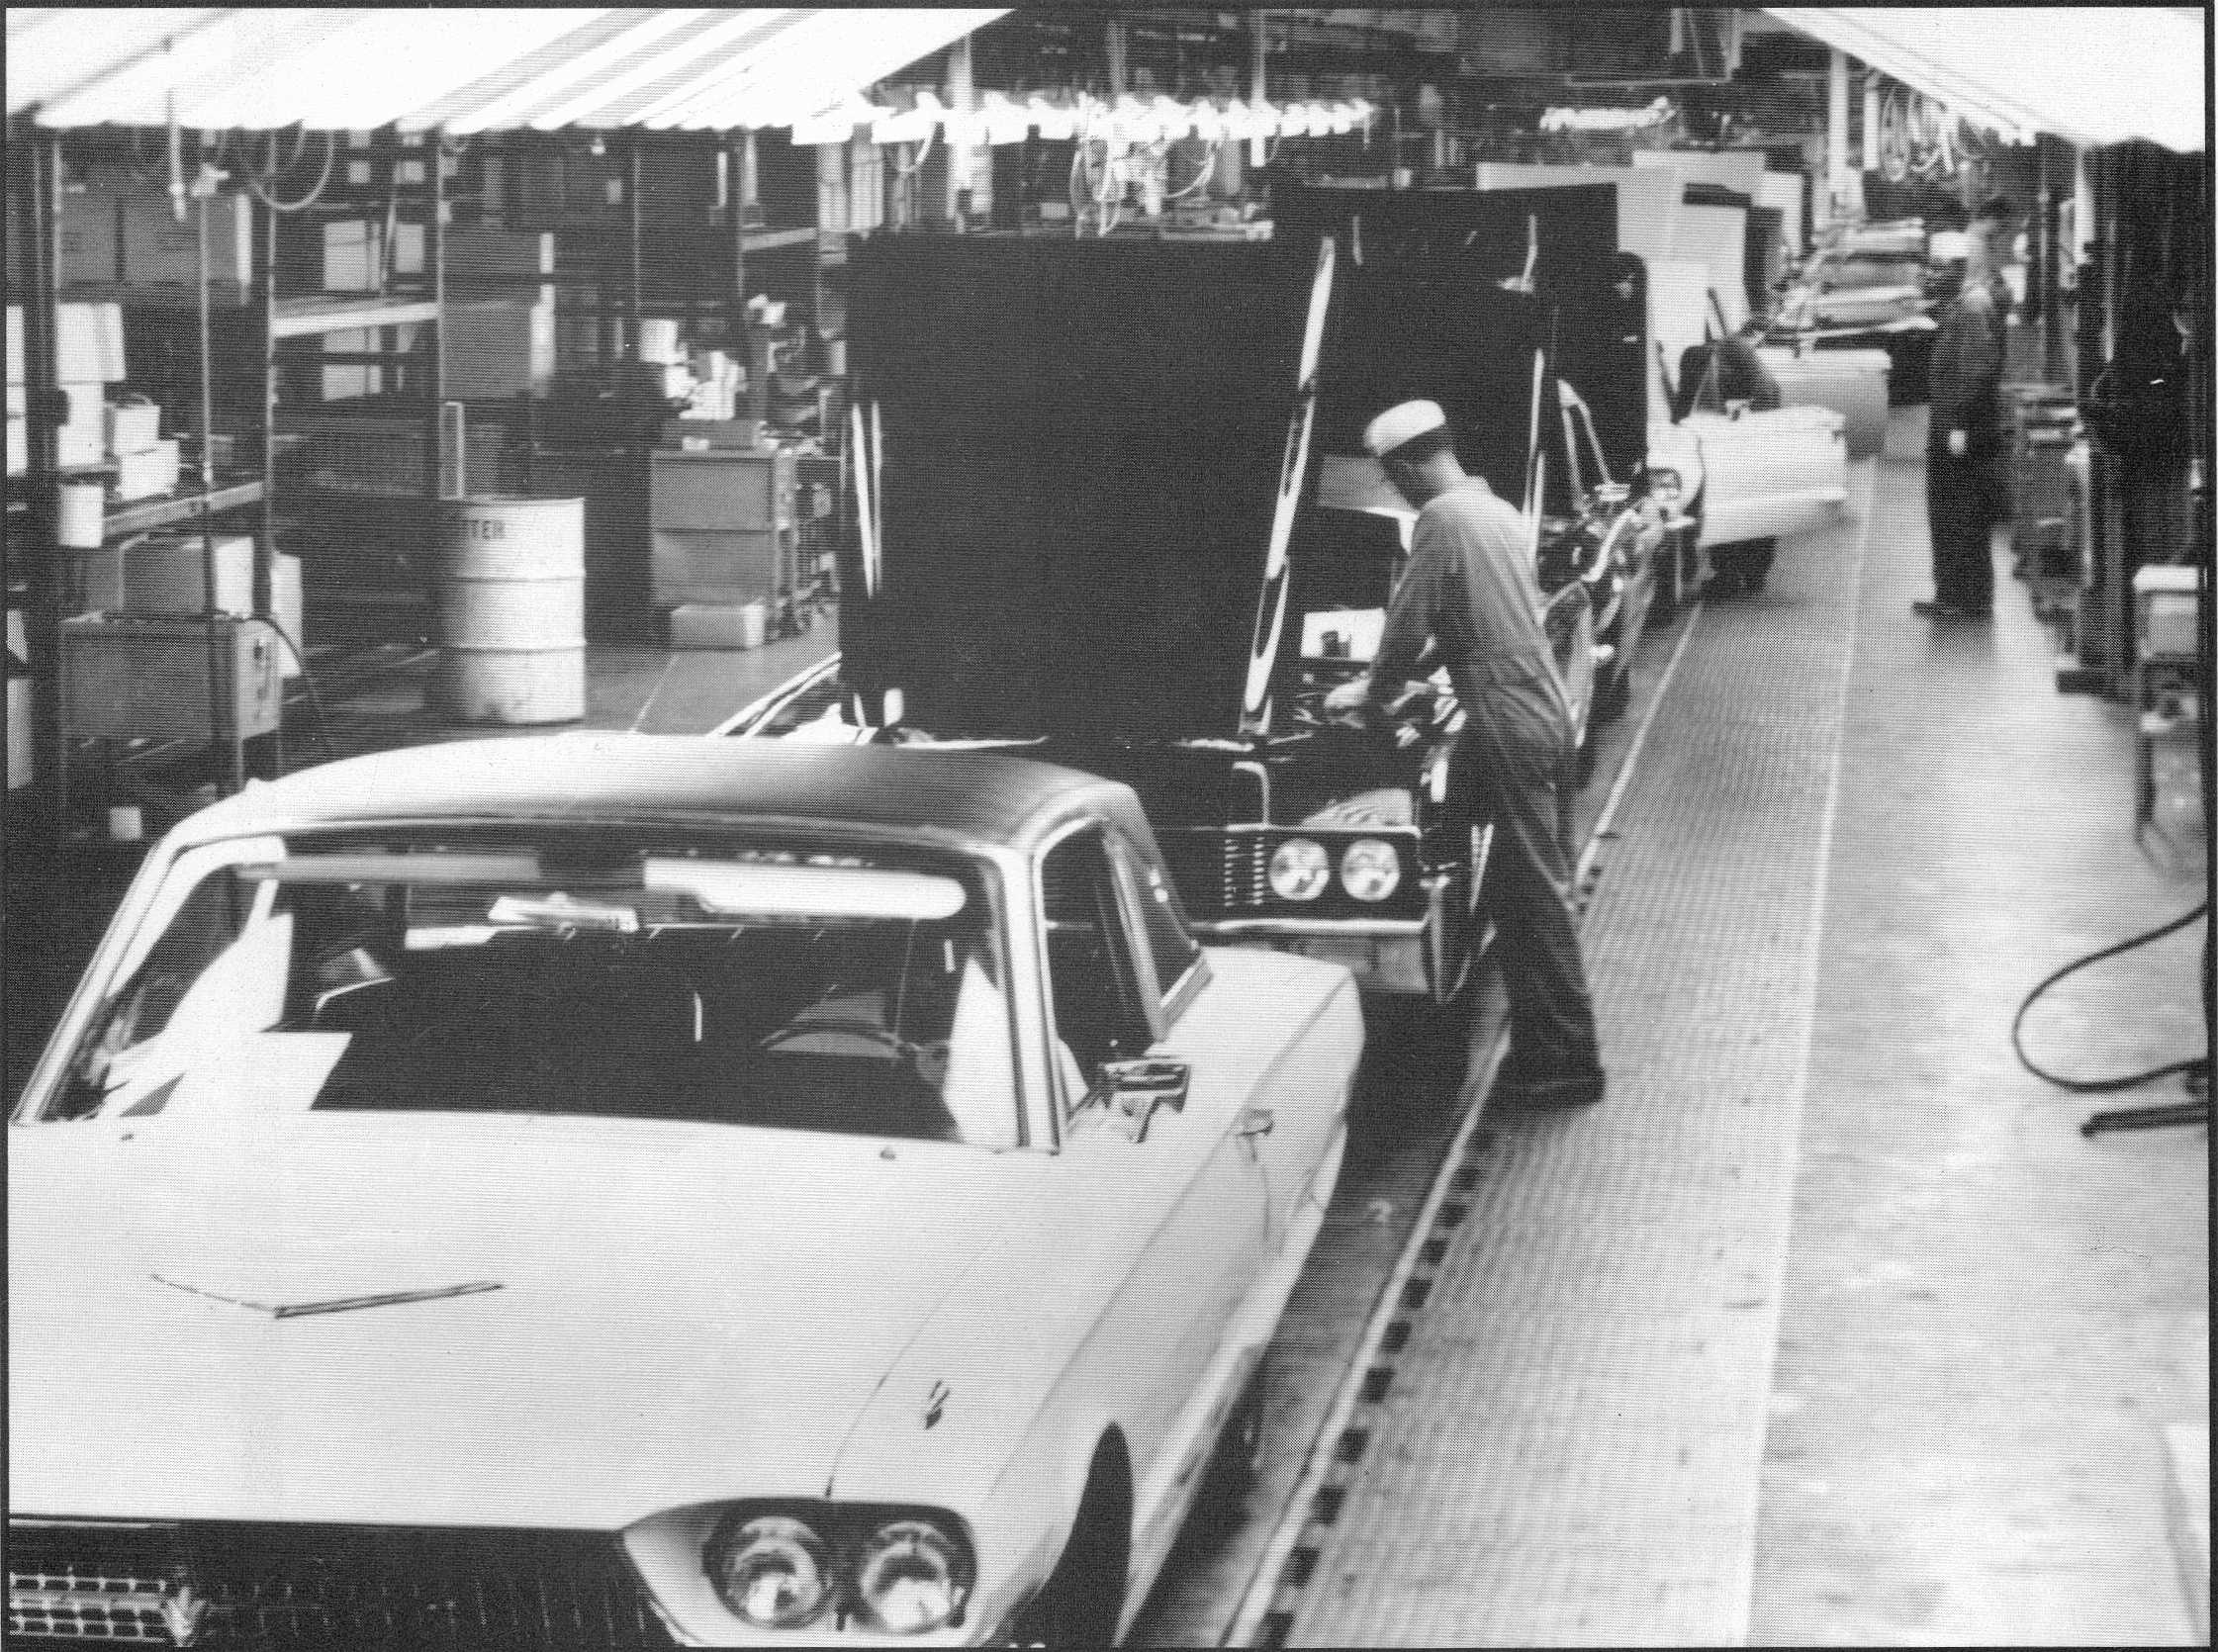
\includegraphics[width=\textwidth]{figs/assembly-line.jpg}
%      
%      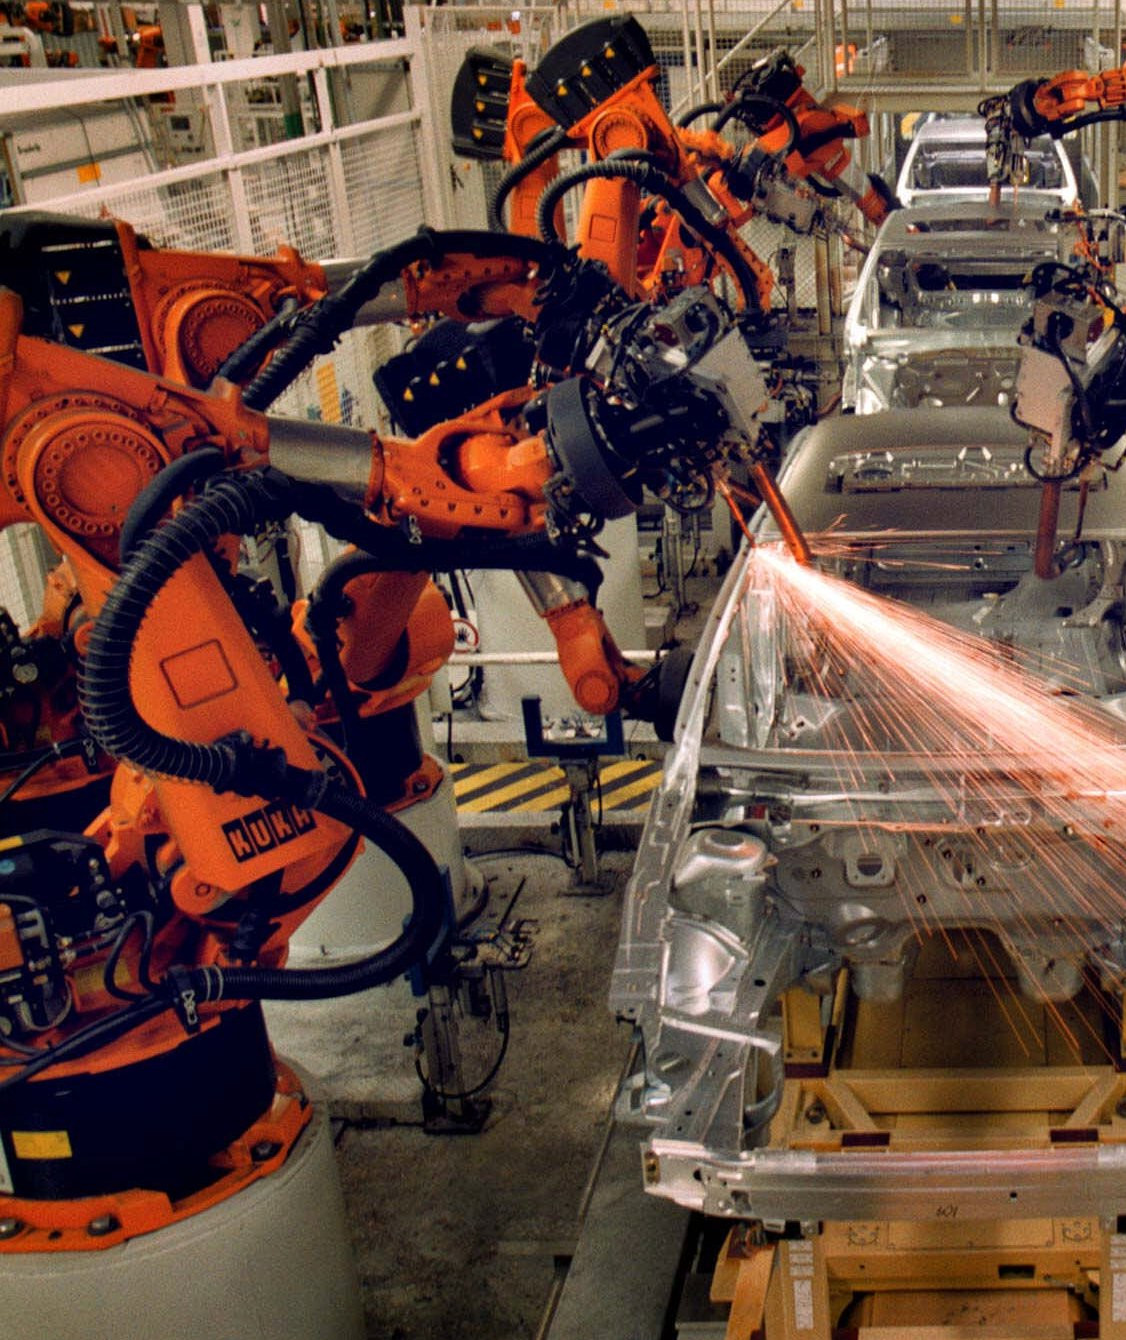
\includegraphics[width=\textwidth]{figs/car-robots.jpg}
%      \end{center}
%      \caption{Something}
%   \end{subfigure}
%   \begin{subfigure}[b]{0.24\textwidth}
%      \begin{center}
%      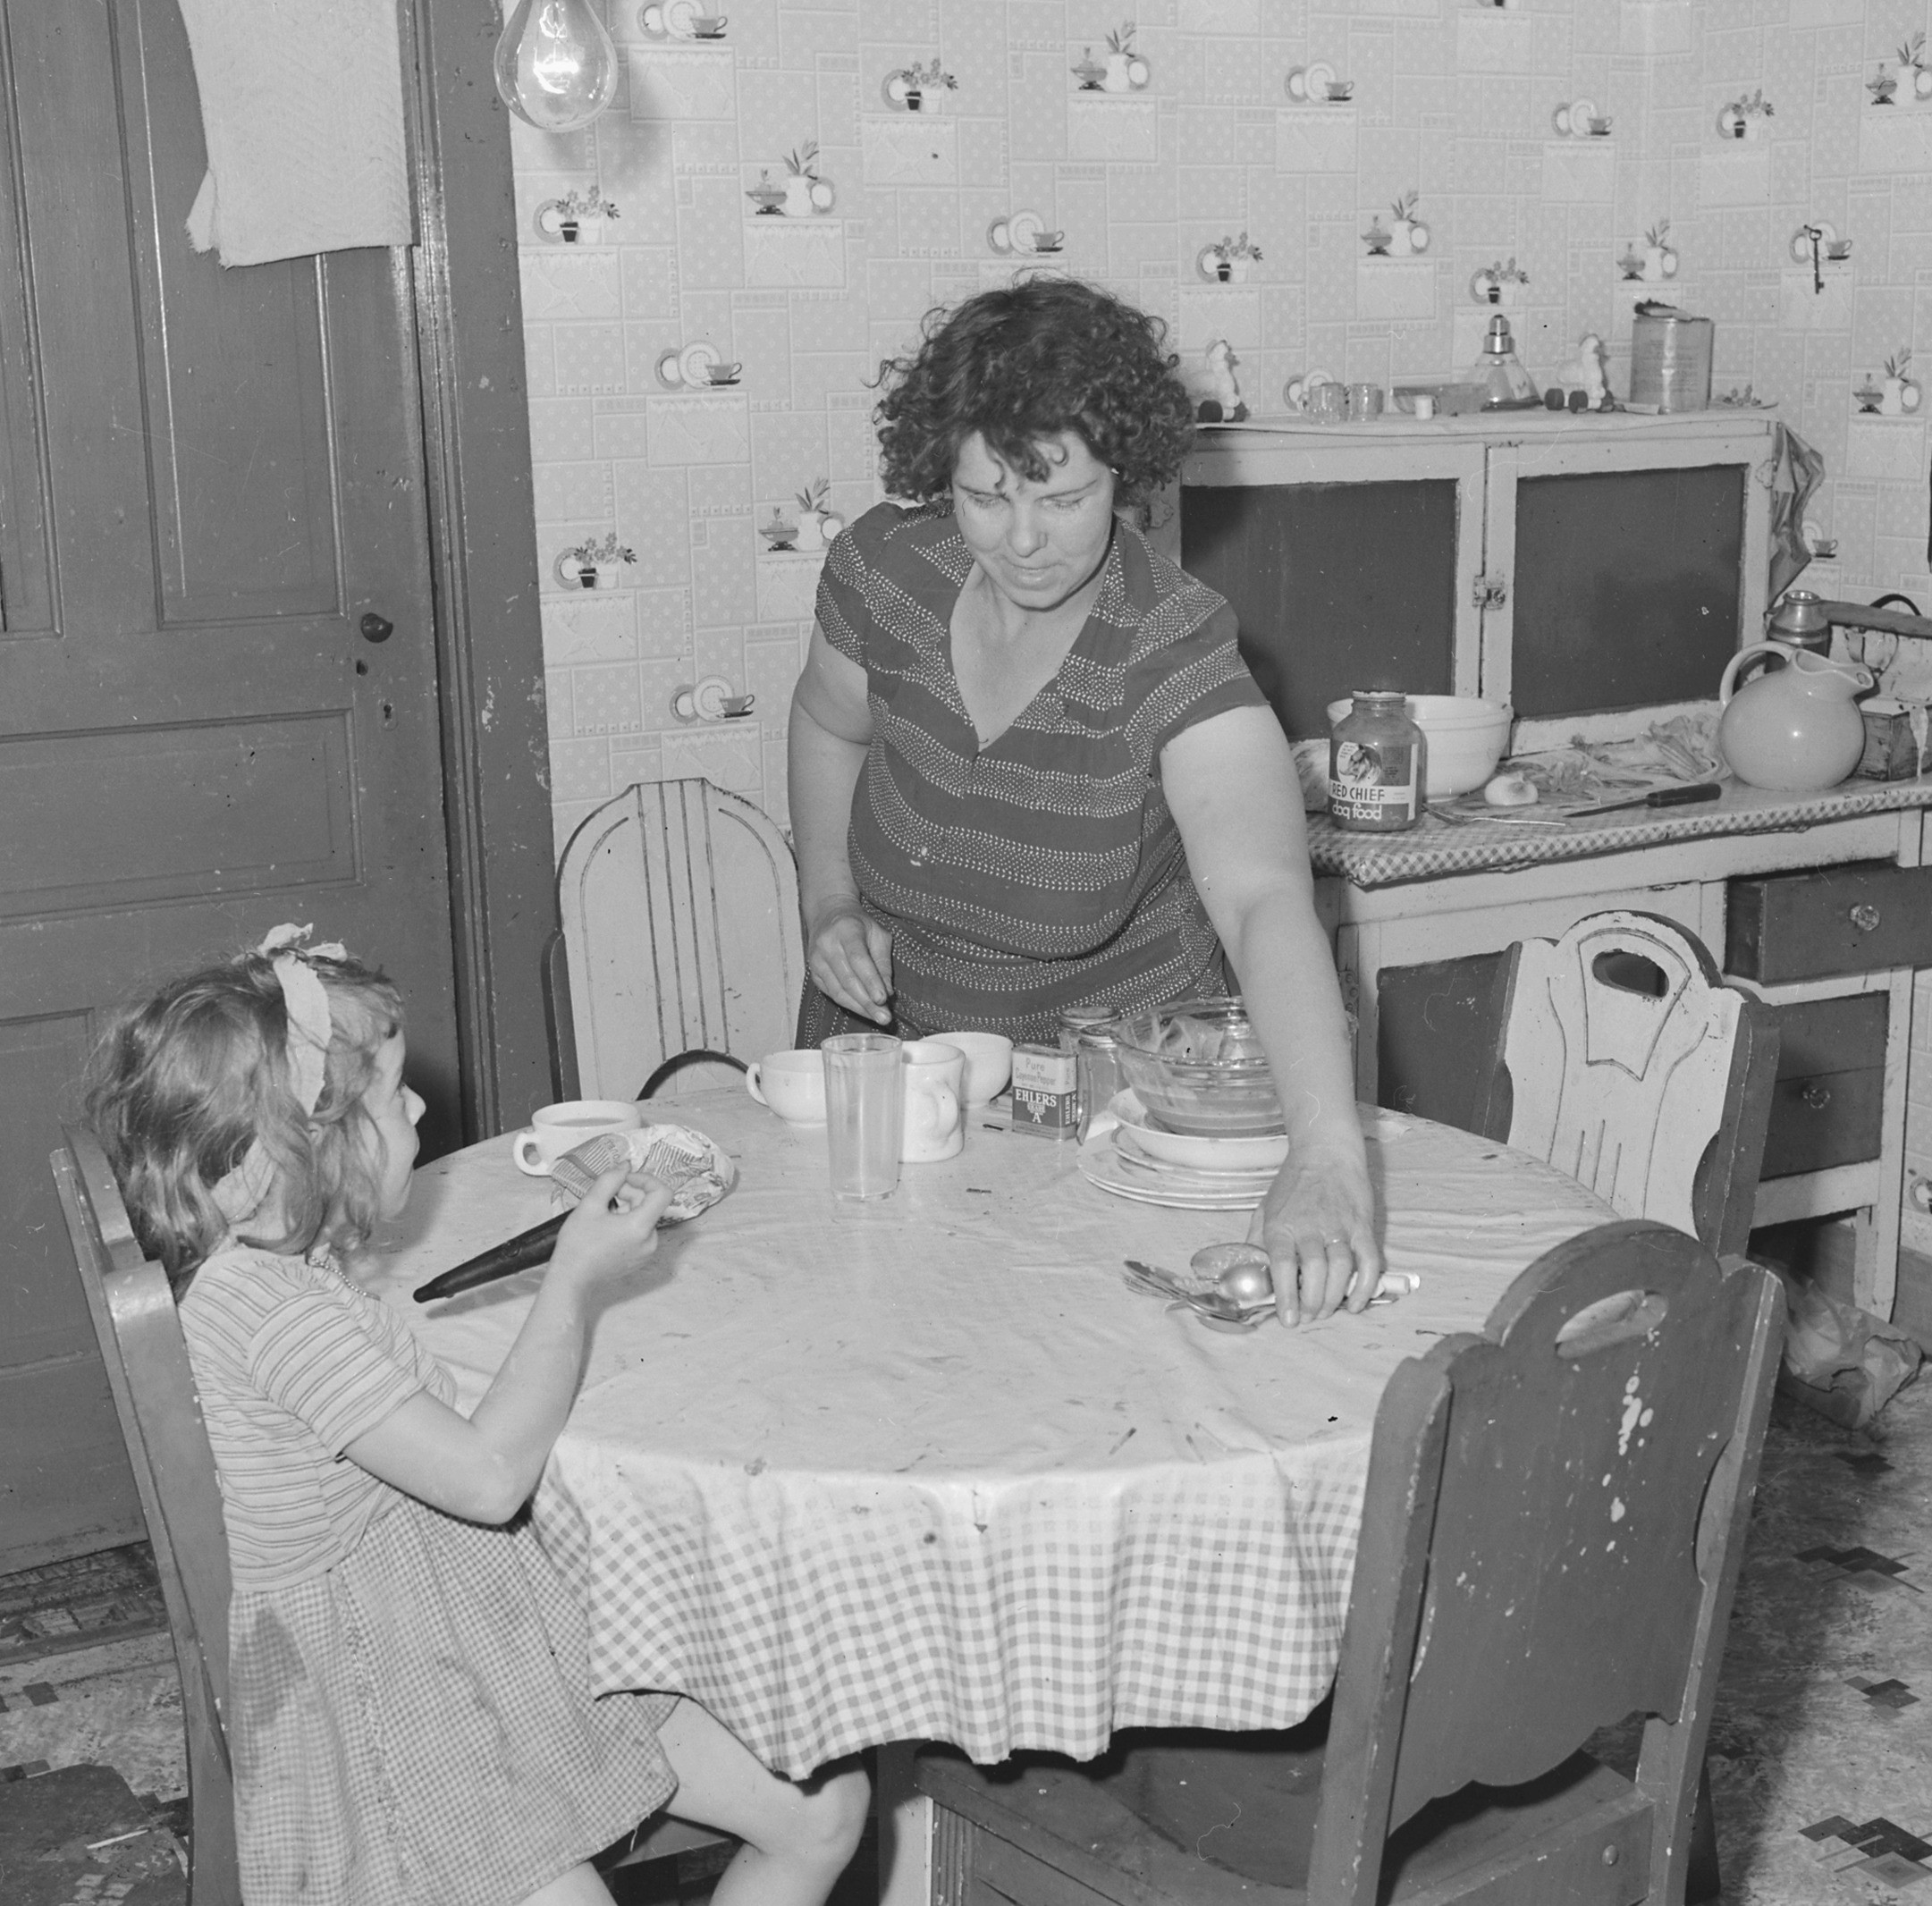
\includegraphics[width=\textwidth]{figs/table-clearing.jpg}
%      
%      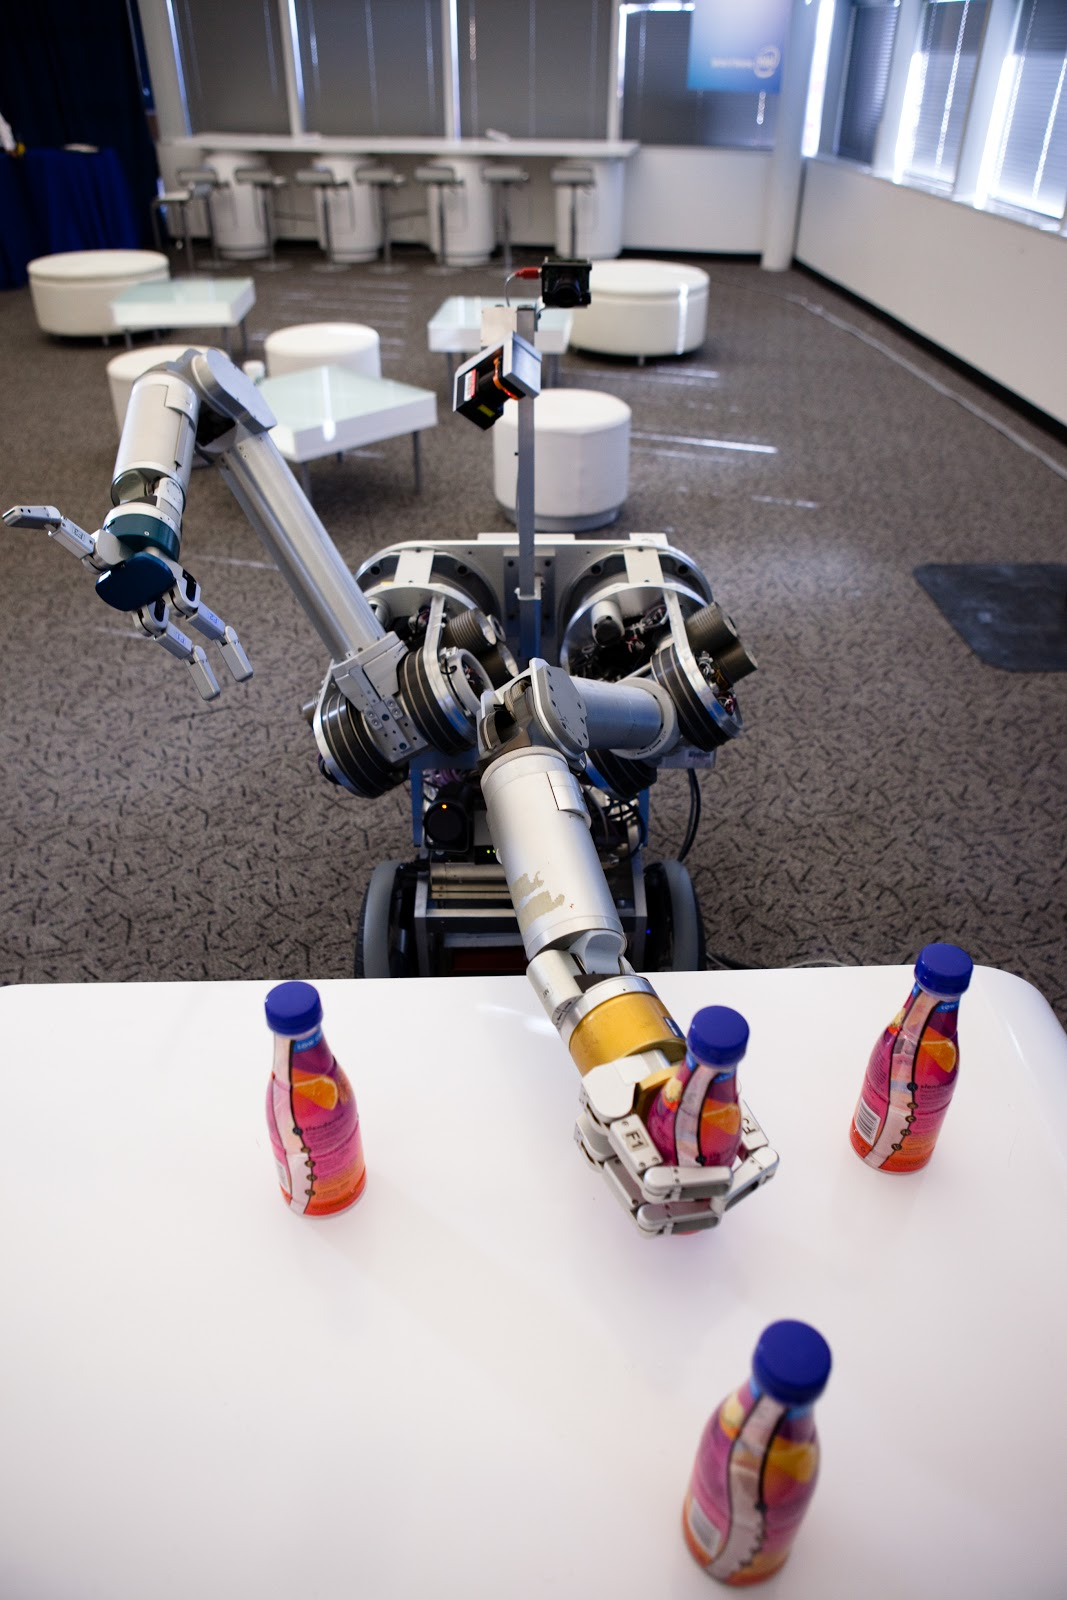
\includegraphics[height=2in]{figs/herb-fuze.jpg}
%      \end{center}
%      \caption{HERB Robot}
%   \end{subfigure}
%   \begin{subfigure}[b]{0.24\textwidth}
%      \begin{center}
%      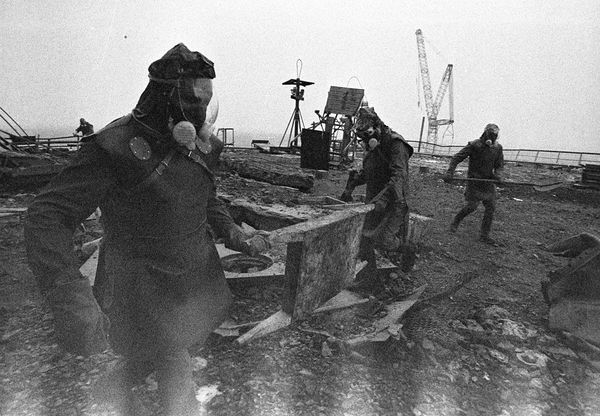
\includegraphics[width=\textwidth]{figs/chernobyl.jpg}
%      
%      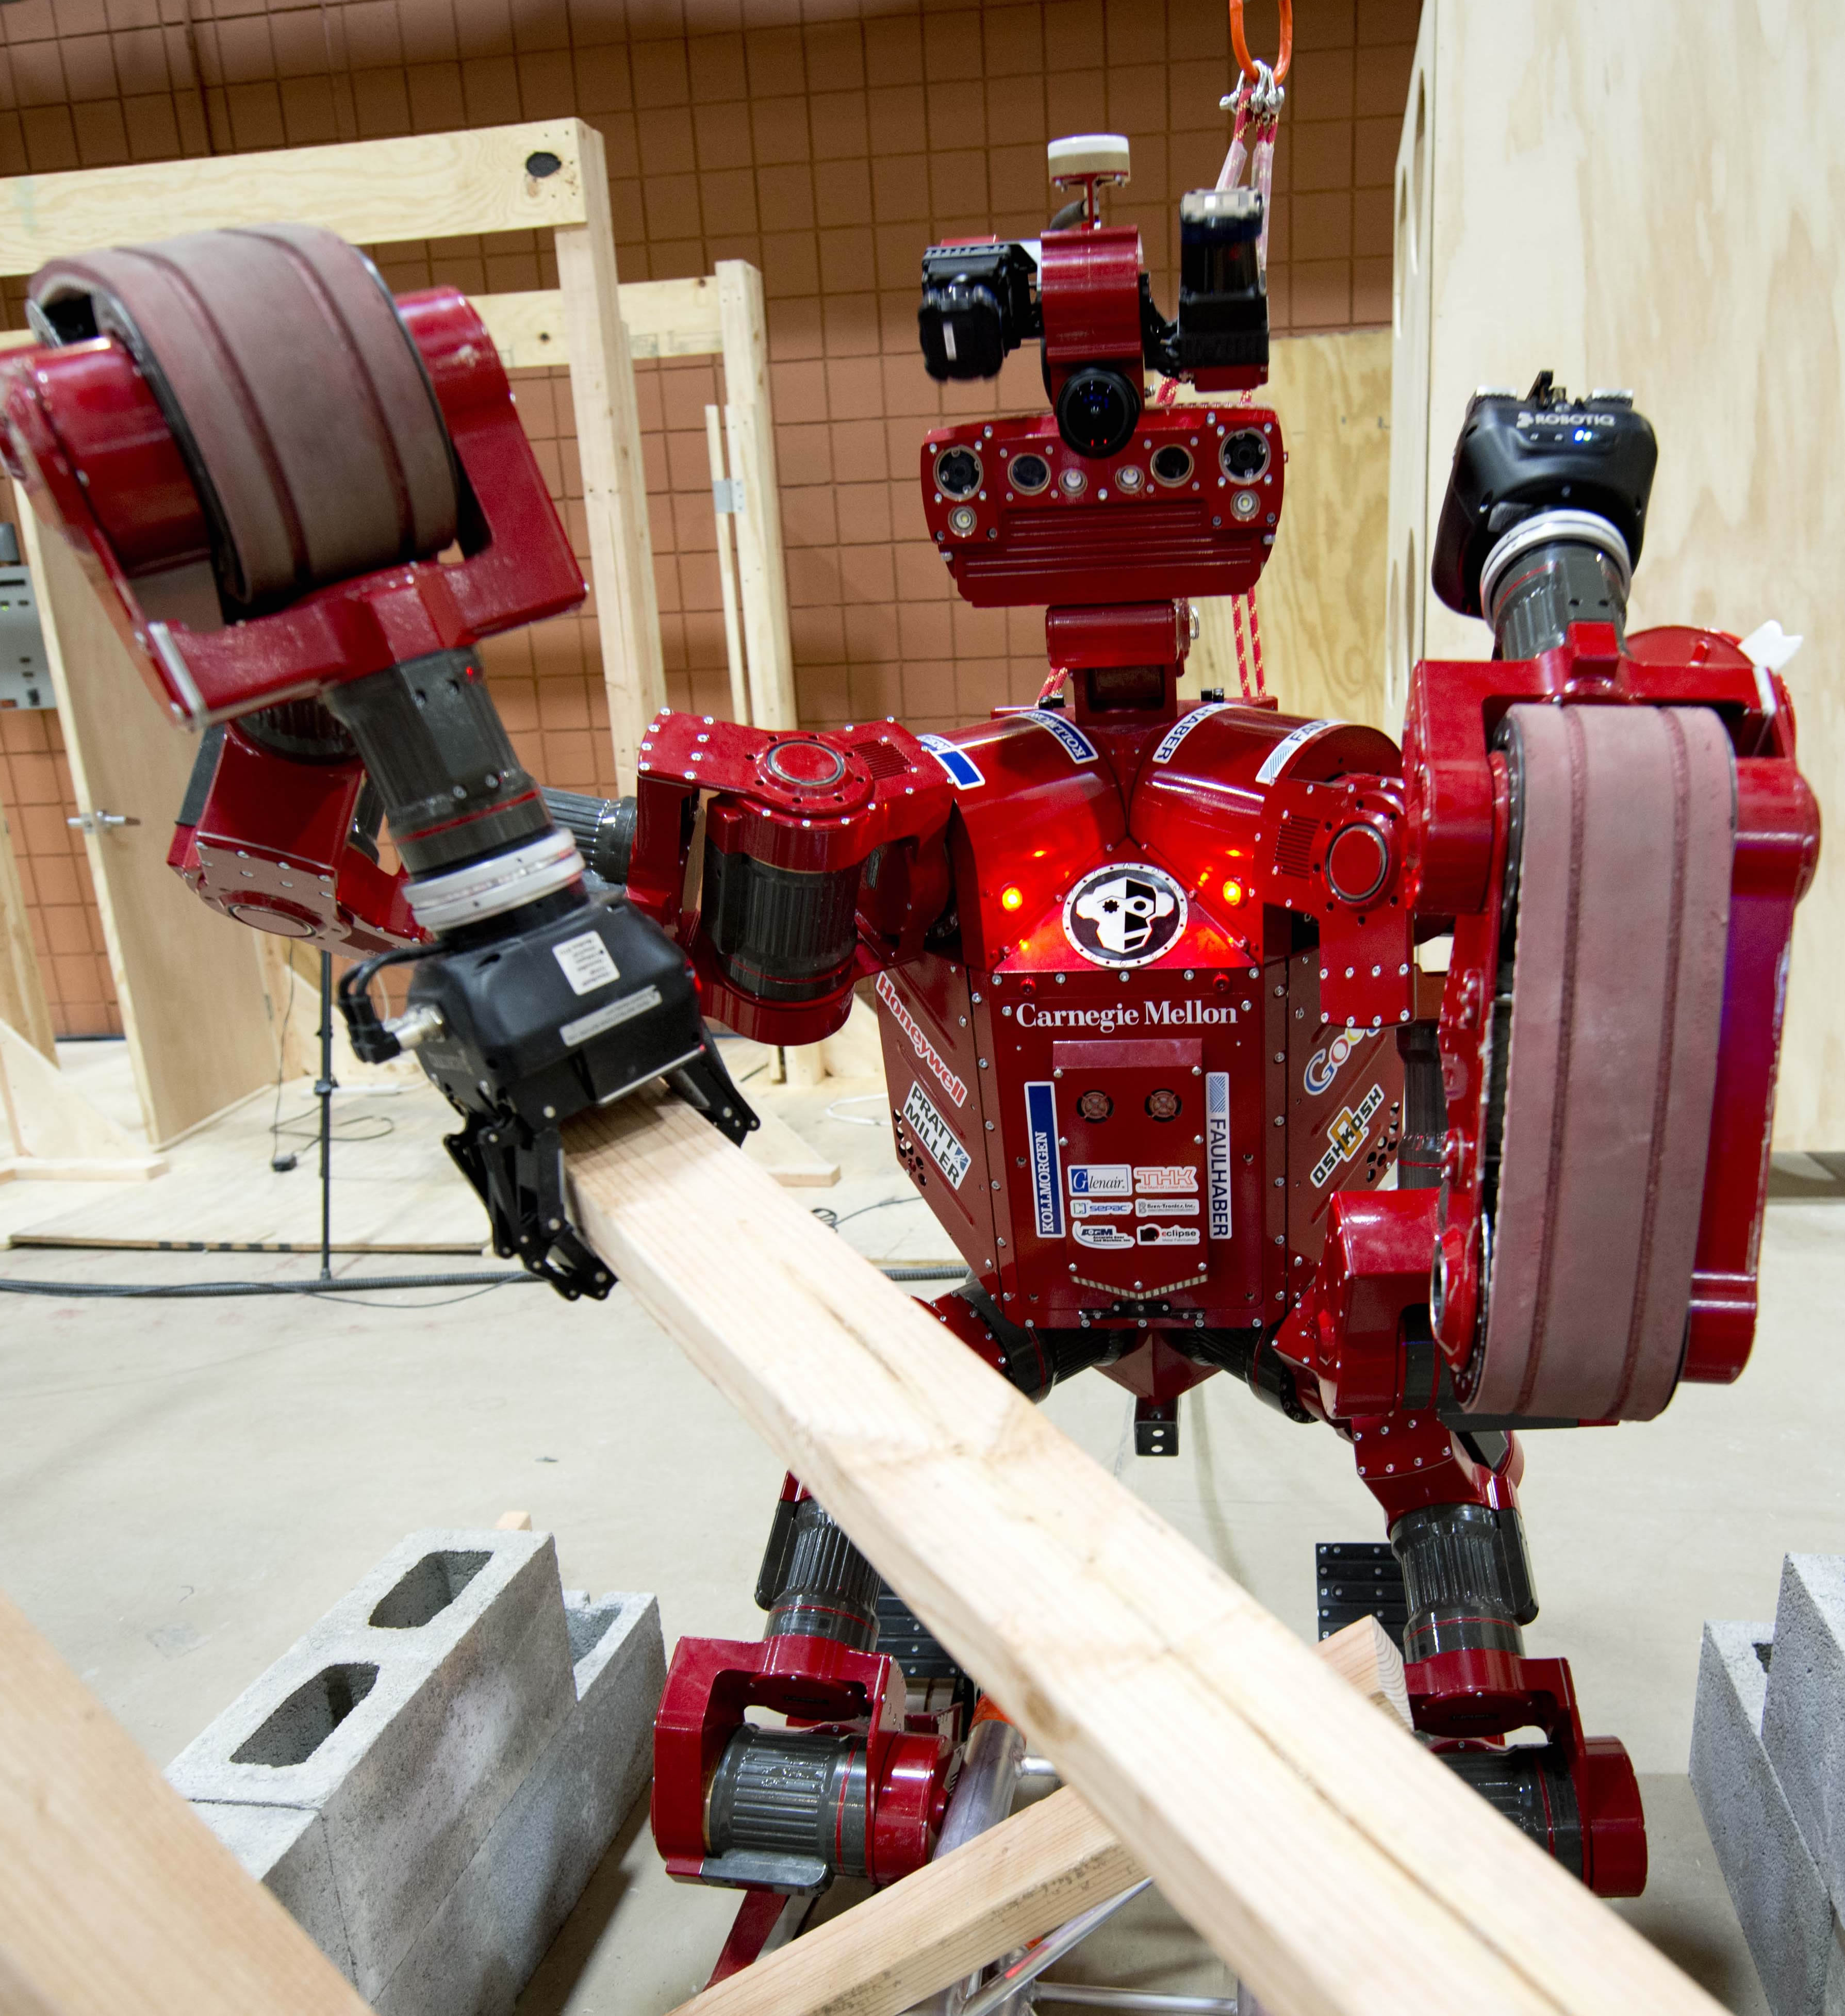
\includegraphics[height=2in]{figs/chimp-debris.jpg}
%      \end{center}
%      \caption{CHIMP Robot}
%   \end{subfigure}
%   \caption{Manipulation problems.}
%\end{widepage}
%\end{figure}
